%% paper.tex


%\documentclass[pldi]{sigplanconf-pldi16}
\documentclass[preprint]{sigplanconf-eurosys}
% standard LaTeX packages

% standard LaTeX packages
%\usepackage{changebar}

\usepackage{balance}
\usepackage{alltt}
\usepackage{amsmath}
\usepackage{balance}
\usepackage{booktabs}
\usepackage{fixltx2e}
\usepackage{graphicx}
\usepackage{boxedminipage}
\usepackage{hyperref}
\usepackage{nicefrac}
\usepackage{subfig}
\usepackage{xcolor}
\usepackage{setspace}
\usepackage{xspace}
\usepackage{multirow}
\usepackage{colortbl}
\usepackage{amsfonts} 
\usepackage{blindtext}
\usepackage{chngpage}
\usepackage{listings}
\usepackage{mathtools}
\usepackage{amssymb}
\usepackage{pifont}
%\usepackage{pgfplotstable}

\usepackage[linesnumbered, vlined, ruled]{algorithm2e}
% font selection
%\usepackage{courier}
%\usepackage[scaled]{helvet}
\usepackage{mathptmx}
\usepackage{times}

% custom packages for this paper
%\usepackage{double-blind}
\usepackage{shared-affiliation}

\usepackage[numbers,sort&compress,square]{natbib}
%\newcommand{\wenfei}[1]{\textcolor{red}{$<<$Wenfei: #1$>>$}}

\lstset{
  basicstyle=\tiny,
  columns=fullflexible,
  numbersep=5pt,
  numberstyle=\scriptsize,
  showstringspaces=false,
  escapeinside={/*@}{@*/},
  belowcaptionskip=1\baselineskip,
  language=C,
  showstringspaces=true,
  keywordstyle=\bfseries,
  commentstyle=\itshape,
}


%\pgfplotstableset{
%    color cells/.style={
%        col sep=comma,
%        string type,
%        postproc cell content/.code={%
%                \pgfkeysalso{@cell content=\rule{0cm}{2.4ex}\cellcolor{black!##10}\pgfmathtruncatemacro\number{##1}\ifnum\number>5\color{white}\fi##1}%
%                },
%        columns/x/.style={
%            column name={},
%            postproc cell content/.code={}
%        }
%    }
%}


\makeatletter
\def\@copyrightspace{\relax}
\makeatother

\captionsetup{format=default, font=bf}


\newcommand*{\Scale}[2][4]{\scalebox{#1}{$#2$}}%
\newcommand{\comment}[1]{{}}



%% taken from unknown.sty
%\DeclareCaptionType{copyrightbox}

\sloppy

\input macros.tex

\begin{document}



\title{
  Characterizing and Predicting which Malwares Get Detected
}

%\numberofauthors{2}
\authorinfo{Paper ID: XXX}
           {Total Page: XXX}

\maketitle


%\theoremstyle{definition}
\newtheorem{definition}{Definition}[section]


\begin{abstract}
\input section/abstract.tex
\end{abstract}


\section{Introduction}

As a free online service, VirusTotal~\cite{virustotal} analyzes files submitted by real-world users to identify many different kinds of malwares, 
like viruses, worms, trojans, and so on. 
VirusTotal applies different antivirus engines to each submitted file and generate an aggregated reports. 
All submitted files and generated reports are saved and can be accessed through public API. 

The repository on VirusTotal provides a good source to conduct data mining. 
Firstly, there are huge amount of data on VirusTotal.
Figure~\ref{fig:subnum} shows that there were more than 40 million suspicious files 
submitted last November. 
This amount of data makes VirusTotal a rough estimation of malwares in the real world. 
Secondly, all data on VirusTotal are labeled by state-of-the-art antivirus techniques. 
VirusTotal updates each antivirus engine every 5 minutes. 
Besides whether a given a submitted file is detected by an antivirus engine, VirusTotal also keeps exact detection tag returned by each engine. 
There are also online active malware researchers, 
who can comment and vote each submitted file and serve as an important supplement of antivirus engines. 
We believe mining data on VirusTotal could enable many ``Big Security'' applications. 

In industry, antivirus vendors widely use VirusTotal to identify false negatives and false positives of their products. 
They only utilize VirusTotal reports separately for each single suspicious file, but fail to leverage the whole repository. 
In academia, researchers began to pay attention to correlations among different VirusTotal reports. 
For example, {\bf [ToDo: discuss Heqing's work]}
We believe there are much more research opportunities through mining VirusTotal. 

In this paper, we view data on VirusTotal as a stream, based on each file’s submission time, and design two stream mining applications: 
\textit{hot malware family mining} and \textit{malware prediction}. 
There are possibly infinite malware families. 
Hot malware family mining can precisely identify malware families, 
which occupy more than a given percentage of total malwares, by using a constant number of counters.
Malwares does not appear uniformly across different malware families or across time, 
and they appear in bursts. 
We built a cache-based algorithm to predict malwares in which families would appear in the near future. 

\begin{figure}[t!]
\begin{center}
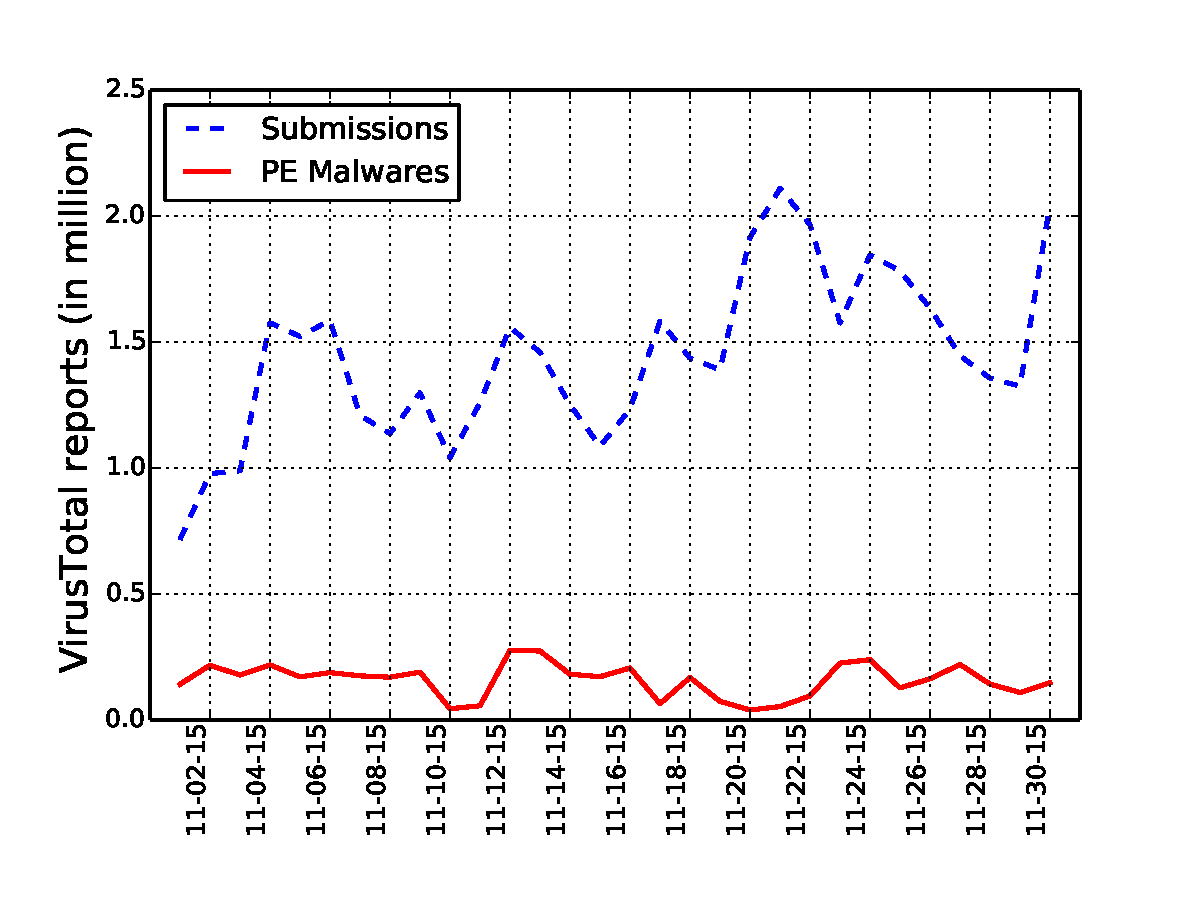
\includegraphics[width=3.0in]{figure/nov}
\caption{The number of files submitted to VirusTotal last November. }
\label{fig:subnum}
\end{center}
\end{figure}

In summary, we made the following contributions in this paper:

\begin{itemize}

\item We collect data submitted to VirusTotal last November, 
and briefly analyze these data to understand the characteristics of VirusTotal repository (Section~\ref{sec:meth}). 
\item We build two stream mining applications, one could identify hot malware family in a constant number of counters (Section~\ref{sec:hot}), 
and the other could predict malwares in the near future (Section~\ref{sec:predict}). 
Experimental results show that we can cover all hot malware family with a very few false positives, and we can predict future malwares with a high precision.
\item We discuss the future research opportunities through mining data on VirusTotal (Section~\ref{sec:oppo}), 
and demonstrate the feasibility by using our experience of building stream mining applications. 

\end{itemize}




\section{Data Collection}
\label{sec:meth}


In this section, we discuss how we collect and preprocess data from VirusTotal. 



\begin{figure*}[!htb]
\minipage{0.31\textwidth}
  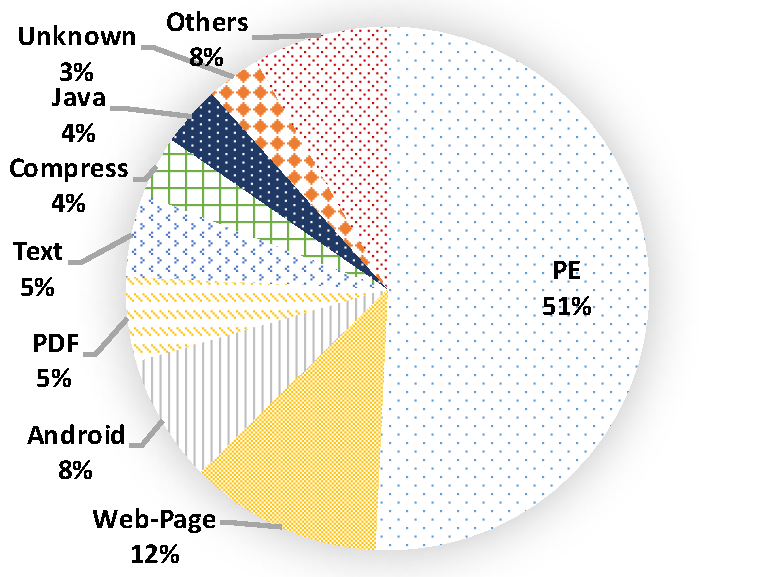
\includegraphics[width=\linewidth]{figure/type}
  \mycaption{fig:type}{File types for all submissions.}
{\footnotesize{(File types and their distributions for all VirusTotal submissions from 05/07/2016 to 09/06/2016.)}}
  %\label{fig:overlap}
\endminipage\hfill
\minipage{0.31\textwidth}
  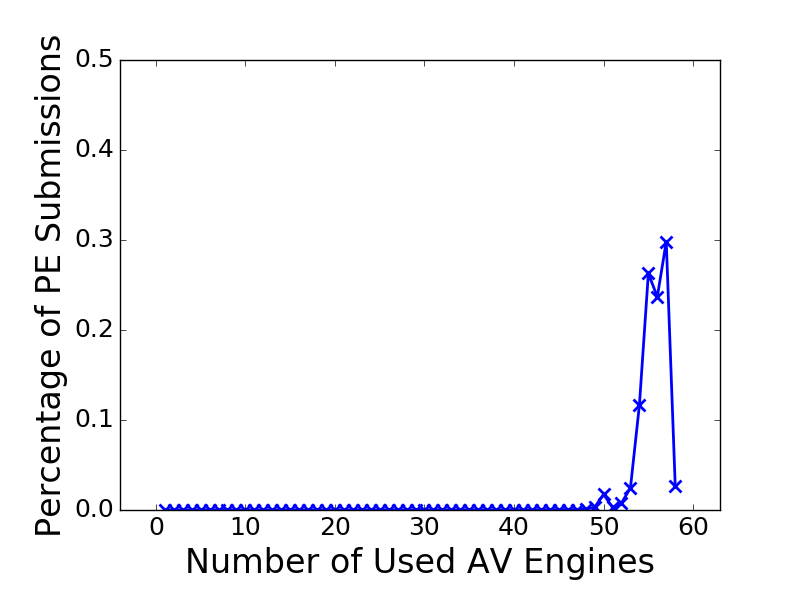
\includegraphics[width=\linewidth]{figure/numVendor}
  \mycaption{fig:vendornum}{The distribution for the number of used anti-virus engines.}
  {\footnotesize{(How the number of used anti-virus engines distributes among all PE submissions we collect.)}}
  %\label{fig:maxUncover}
\endminipage\hfill
\minipage{0.31\textwidth}%
  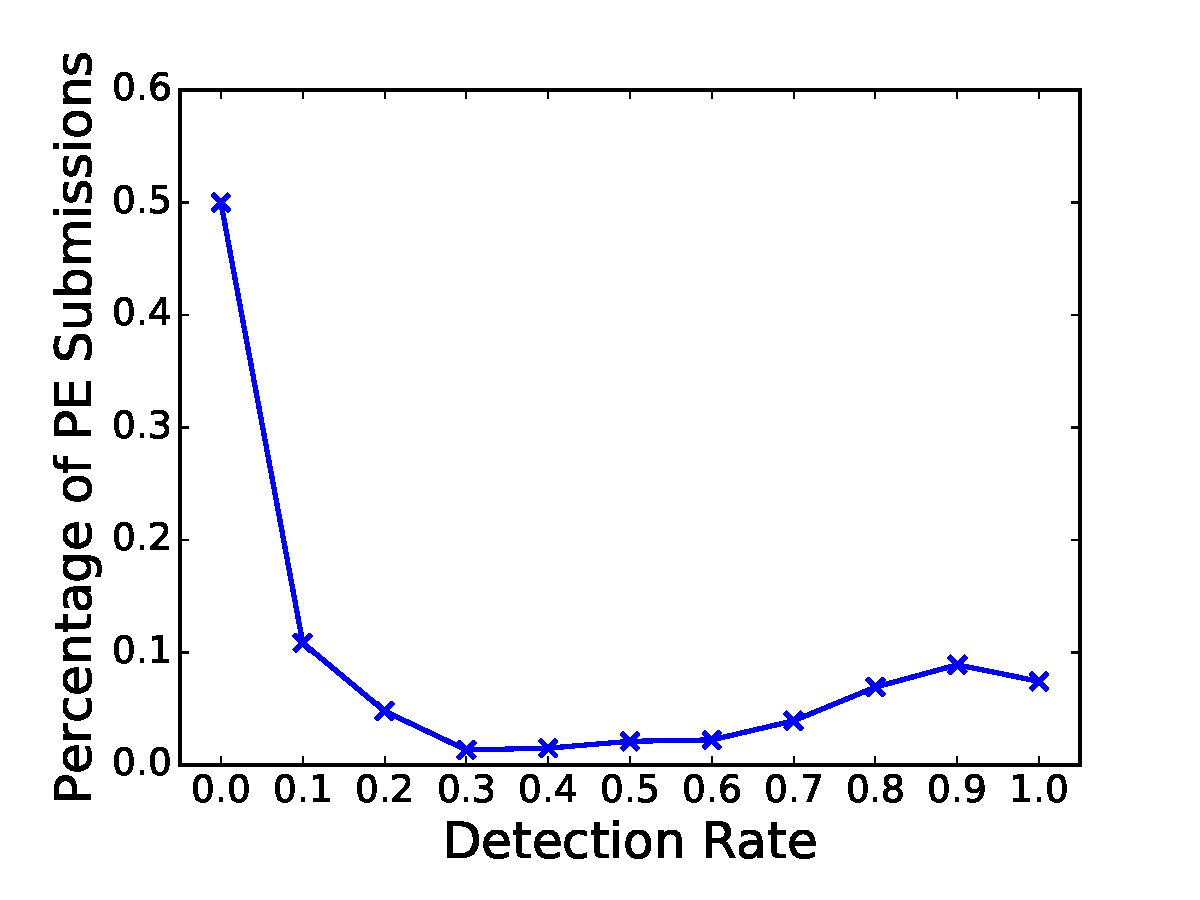
\includegraphics[width=\linewidth]{figure/DetectionRate}
  \mycaption{fig:detectiorate}{The distribution for detection rate.}
{\footnotesize{(How detection rate distributes among all PE submissions we collect. 
Each detection rate is rounded up to nearest 0.05.)}}
  %\label{fig:aveUncover}
\endminipage\hfill

%\vspace{-0.2in}
\end{figure*}


\begin{table}[h!]
\centering
\footnotesize
{
%\begin{tabular}{@{\hspace{3pt}}l@{\hspace{3pt}}|@{\hspace{3pt}}c@{\hspace{3pt}}}
\begin{tabular}{l|l}
\hline
Metadata Field & Explanation \\
\hline                            
%\cline{1-1}
{\bf name}      & submitted file name \\
{\bf link}      & where to download the file \\
{\bf timestamp} & timestamp when the submission was made \\
{\bf source\_country} & the country where the submission was made \\
{\bf source\_id} & user ID making the submission\\
{\bf size} & file size \\
{\bf type} & file type \\
{\bf tags} & labels with more specific information for each {\bf type}\\
{\bf first\_seen} & when the same file was first submitted \\
{\bf last\_seen} & when the same file was last submitted \\
{\bf hashes} & sha1, sha256, md5, and vhash\\
{\bf ssdeep} & ssdeep information digest string \\
{\bf total} & number of engines analyzing the file \\
{\bf positives} & number of engines that flagged the file as malicious \\
{\bf positives\_delta} & changes in {\bf positives} across different submissions\\
{\bf report} & detailed detection report from each AV engine \\
%\multicolumn{2}{|l|}
\hline

\end{tabular}
}
\mycaption{tab:fields}{VirusTotal Metadata.}
{ 
Fields for each submission retrieved from the VirusTotal distribution API and their relation explanation.
The same file can be submitted multiple times by different users.
}
%\vspace{-0.1in}
\end{table}




We collect metadata for each submission through VirusTotal’s distribution API. 
Distribution API keeps returning metadata for latest files submitted to VirusTotal.
Table~\ref{tab:fields} shows the metadata fields and their meaning.  
We began our data collection on May 7th 2016, 
and ended our data collection on September 6th 2016. 
We insert all collected metadata into a cassandra table by using the combination of sha256, source\_id, and timestamp as key.
In total, we collect metadata for 151 million submissions. 

Figure~\ref{fig:type} shows the file type distribution for all submissions. 
Among all file types, \textit{Portable Executable} (PE) files have the largest number, which is the same as results from a previous study~\cite{SongAPsys2016}.
PE files occupy 51\% of all submissions. 
Web pages and malwares on Android have the second and third largest number of malwares, 
occupying 12\% and 8\% of all submissions respectively. 
Other popular file types include PDF, Text, compressed files, and Java files, which is slightly different from the previous study~\cite{SongAPsys2016}. 

Similar to the previous study~\cite{SongAPsys2016}, 
we focus our study in this paper on PE files, 
and leave studies on other types of malwares in the future. 
If the type field for a submission is either ``Win32EXE'' or ``Win32DLL'', 
we consider the submission is a PE file. 
In total, we collect 76 million PE submissions. 
The number of submissions and the number of PE submissions we collected each day are shown in Figure~\ref{fig:subnum}. 

%\begin{figure}[t!]
\begin{center}
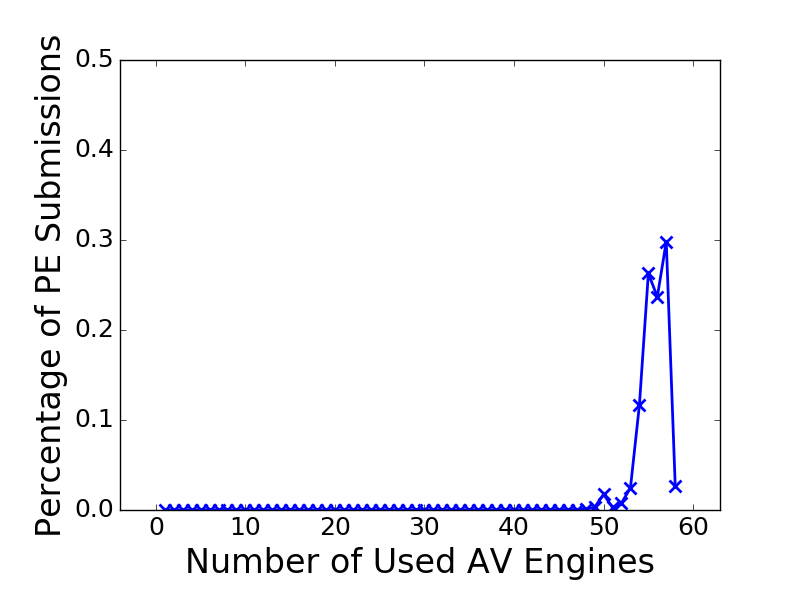
\includegraphics[width=2.5in]{figure/numVendor}
\mycaption{fig:vendornum}{The distribution for the number of used anti-virus engines.}
{
How the number of used anti-virus engines distributes among all PE submissions we collect.
}
\end{center}
%\vspace{-0.25in}
\end{figure}

%\begin{figure}[t!]
\begin{center}
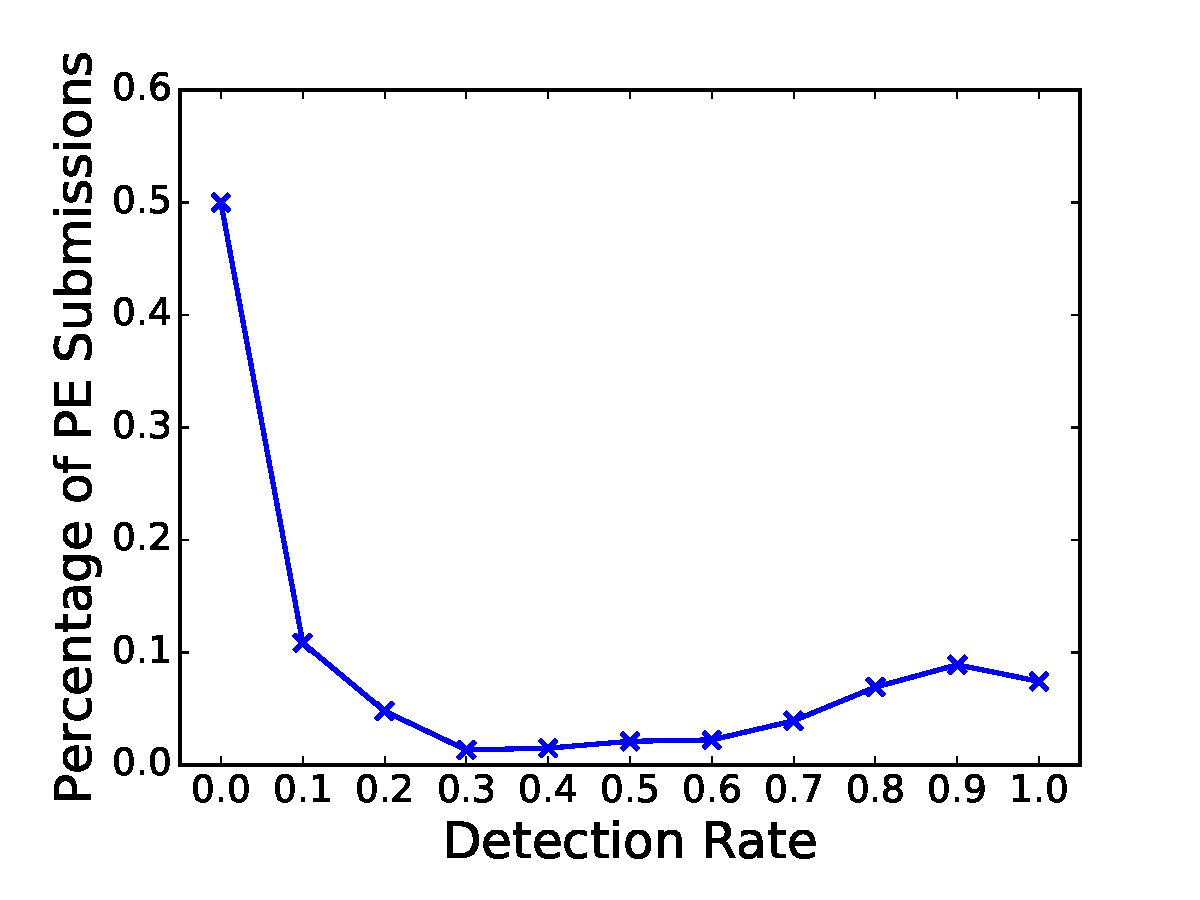
\includegraphics[width=2.5in]{figure/DetectionRate}
\mycaption{fig:detectiorate}{The distribution for detection rate.}
{
How detection rate distributes among all PE submissions we collect.
}
\end{center}
%\vspace{-0.25in}
\end{figure}

For each PE submission, VirusTotal will use a bunch of anti-virus engines to analyze it.
As shown in Table~\ref{tab:fields}, 
total field is to represent the number of used anti-virus engines. 
Figure~\ref{fig:vendornum} shows the distribution for the number of used anti-virus engines. 
More than 99\% of PE submissions are analyzed by at least 50 anti-virus engines. 
Some anti-virus engines will identify a submitted PE file as malware, while others will not. 
Positives field in Table~\ref{tab:fields} represents the number of anti-virus engines identifying the submission as malwares. 
%We calculate detection rate for a submission by using total number to divide positives number. 
%Figure~\ref{fig:detectiorate} shows how detection rate distributes among all PE submissions. 

$$ \textrm{\textit{Detection Rate}} = \dfrac{positives}{total + 1}$$

Detection rate represents the percentage of engines identifying the submission as malware. 
Adding one to total is to avoid dividing 0 exception, and more importantly, 
to give submissions identified by more engines higher detection rate. 
For example, after adding one, submissions analyzed by 50 engines and detected by 50 engines will have a higher detection rate 
than submissions analyzed by 1 engine and detected by 1 engine. 
This formula shares the same intuition from previous work~\cite{GuoICSE2010}, when computing reputations for bug reporters. 
A larger detection rate means more malicious of the malware. 
Figure~\ref{fig:detectiorate} shows how detection rate distributes among all PE submissions. 


One PE file could be submitted more than once to VirusTotal. 
There are 6.72\% PE files submitted more than once to VirusTotal. 
On average, each PE file is submitted 1.19 times. 
Some anti-virus engines may change their results when analyzing the same file during different submissions.
We will discuss how vendors influence each other and how to predict possible detection result change in Section~\ref{sec:influ}.

Like all other empirical study works, 
our findings and conclusions need to be considered with our methodology in mind. 
We use distribution API to download submissions' metadata from VirusTotal. 
There is no guarantee that all data can be successfully downloaded. 
It could be possible that some files are submitted to VirusTotal, 
but we fail to get their information from VirusTotal.
Although we have collected huge amount of malware information from VirusTotal,
we do believe that there are malwares never submitted to VirusTotal, 
or submitted to VirusTotal much later than they appear in the real world. 
However, there are no conceivable ways to study them.
We believe the 4-month malware information we collect can serve as a representative sample for malwares in the real world. 

\section{Influence on Detection Rate}
\label{sec:corr}
In this section, we study factors influencing detection rate of PE submissions. 
Our study is conducted from 4 aspects: reputation of source id, submission history, 
file size, and source country.

\subsection{Reputation of Source ID}



\begin{figure}[t!]
\begin{center}
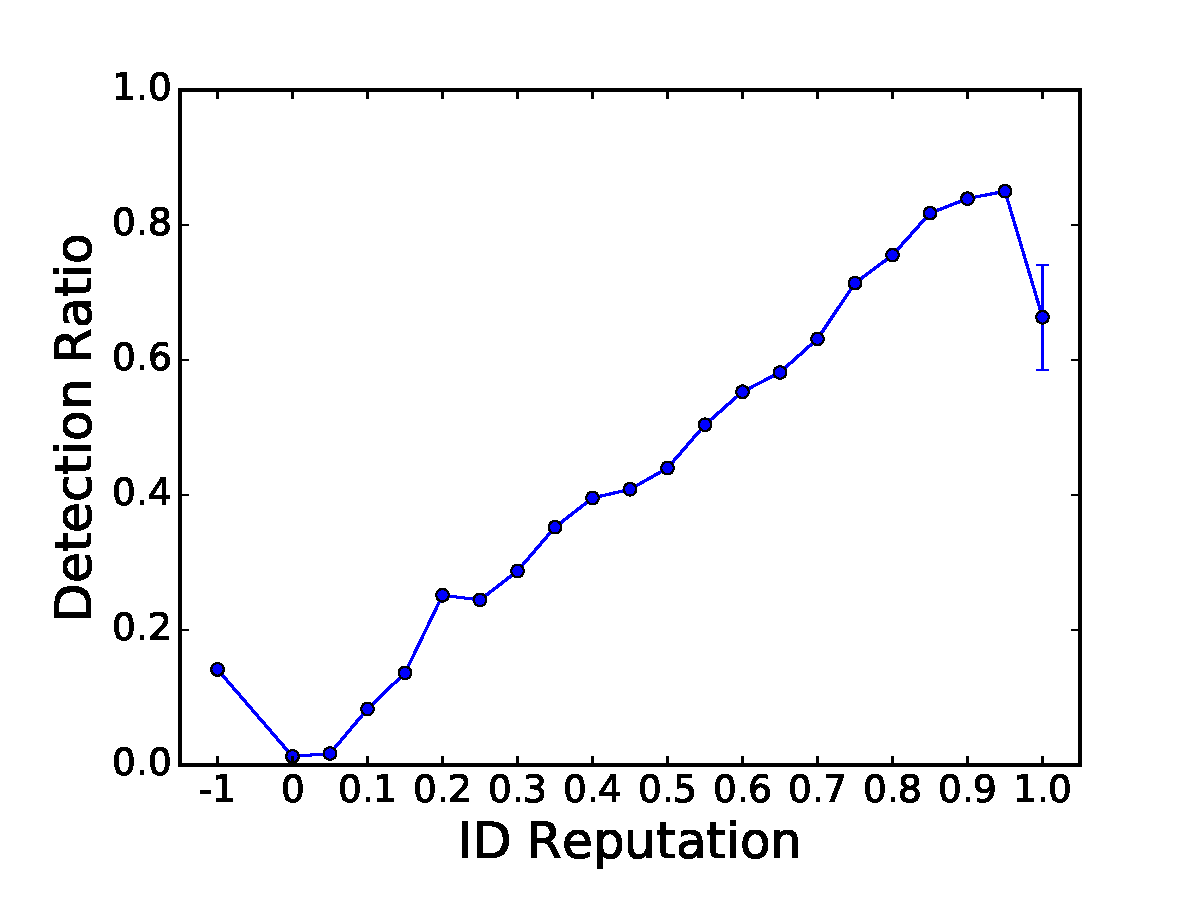
\includegraphics[width=2.5in]{figure/IDReputation}
\mycaption{fig:idreputation}{The relation between source id's previous reputation and detection rate.}
{\footnotesize{(How detection rate changes with the value of source id's reputation. Each reputation is rounded up to nearest 0.05.
Reputation -1 means the source id did not make any submission before. 95\% confidence interval is also drawn 
for each point.)}}
\end{center}
%\vspace{-0.25in}
\end{figure}


Previous work~\cite{GuoICSE2010} reported correlation between bug reporter’s reputation and the likelihood for the bug being fixed. 
We also observe correlation between the reputation of source id and submission’s detection rate. 

%\theoremstyle{definition}
\begin{definition}{Reputation:}
Given a submission $S$ with source id $I$, 
we define the reputation of $I$ when conducting the submission $S$ as the average detection rate for all submissions conducted by $I$ before $S$. 
If $I$ did not make any submission before, we define the reputation to be $-1$. 
\end{definition}

For around 14\% PE submissions, VirusTotal fails to provide source id information. 
We filter out these submissions, when computing reputation.
All other PE submissions are conducted by 613 thousand source ids. 
More than half source ids (66\%) only conduct submission once. 
We filter source ids conducting more than 1 million PE submissions in our data set, 
because we think these are anti-virus vendors routinely test their products. 

When calculating reputation, we sort all submissions from the same source id chronologically, 
and calculate reputation for the id when conducting each submission. 
We round up each calculated reputation to nearest 0.05. 
We group submissions based on source ids' reputation when conducting submissions, 
and we plot average detection rate and 95\% confidence interval for each group in Figure~\ref{fig:idreputation}. 
Except the point with reputation 1, all other confidence intervals are invisible.  

As shown in Figure~\ref{fig:idreputation}, 
there is a rough increase for detection rate as the increase of source id's reputation, 
with the exception for the point with reputation -1 and the point with reputation 1. 
It is interesting to observe that first submissions conducted by different source ids have higher 
detection rate than submissions conducted by ids with reputation 0, 
and it is difficult for source ids with highest reputation to keep highest reputation.  

{\bf TODO: ADDING A SMALL DISCUSSION PARAGRAPH}

\subsection{Submission History}
\section{Influence Propagation}
\label{sec:influ}


%\input{related}
%\input{conclusion}

%%\balance
%\begin{spacing}{0.65}

\balance
{
\bibliographystyle{abbrvnat}
\bibliography{security} 
}
%\end{spacing}
\end{document}

% Local variables:
% TeX-PDF-mode: t
% TeX-master: t
% End:

% LocalWords:  Crug cci
